\section{Constrained Solution}

Our last step is to resolve all conflicts occurred in the partial solution. Remind that, the partial solution is just an order of POIs in each partition, it does not include any of actual paths.

\subsection{Problem Statement}

\begin{problem}[Conflict Avoidance Problem]
Given a set of POIs and a bijective mapping $b: V_P \to V_P$. Find a set of paths that does not yield any conflict.
\label{prob:conflict}
\end{problem}

The each bijective mapping represents a valid partitioning on the graph

\subsection{Naive Solution}

A naive solution to the conflict avoidance problem of a pair of paths is to fix one path and find the shortest no-conflict path of the other. The strategy can be used to solved the simple case as in figure \ref{fig:naive_conflict}, we fix the blue path $1 \to 3$ and find a shortest path from $5 \to 6$ without inducing any conflict.

\begin{figure}[h!]
\centering
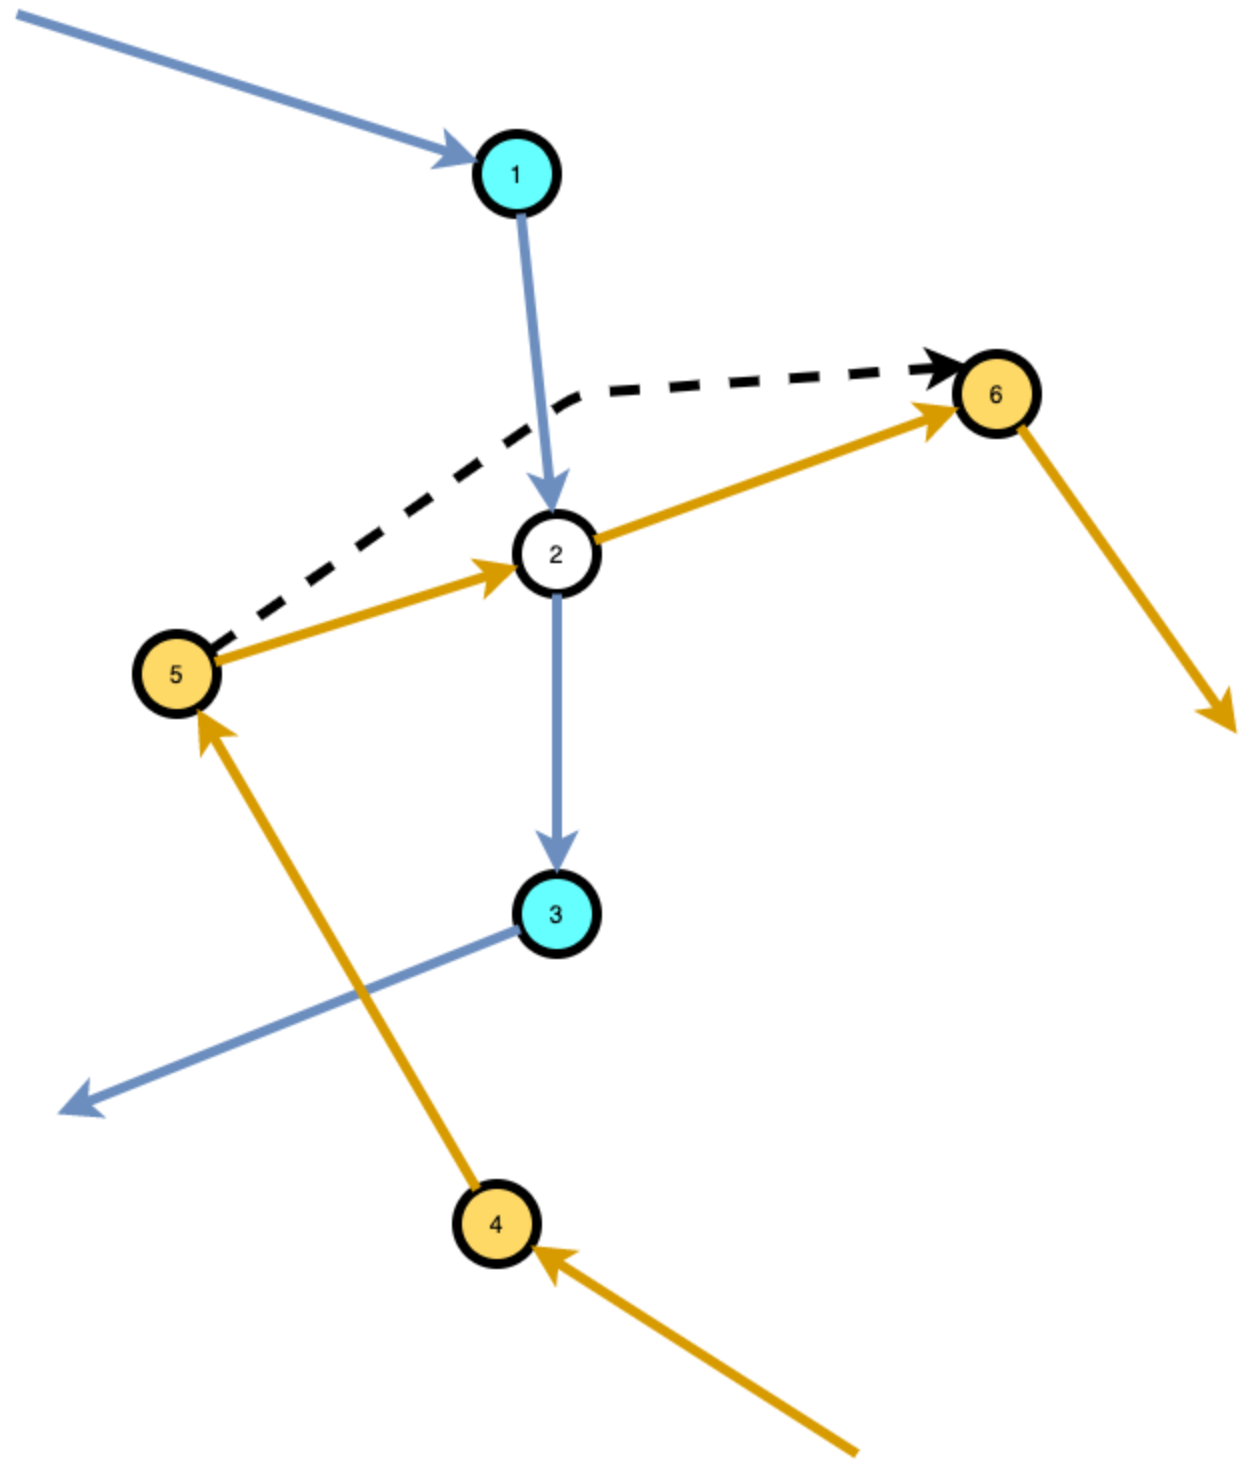
\includegraphics[width=0.8\textwidth]{assets/naive_conflict.png}
\caption{Naive Conflict}
\label{fig:naive_conflict}
\end{figure}

\begin{figure}[h!]
\centering
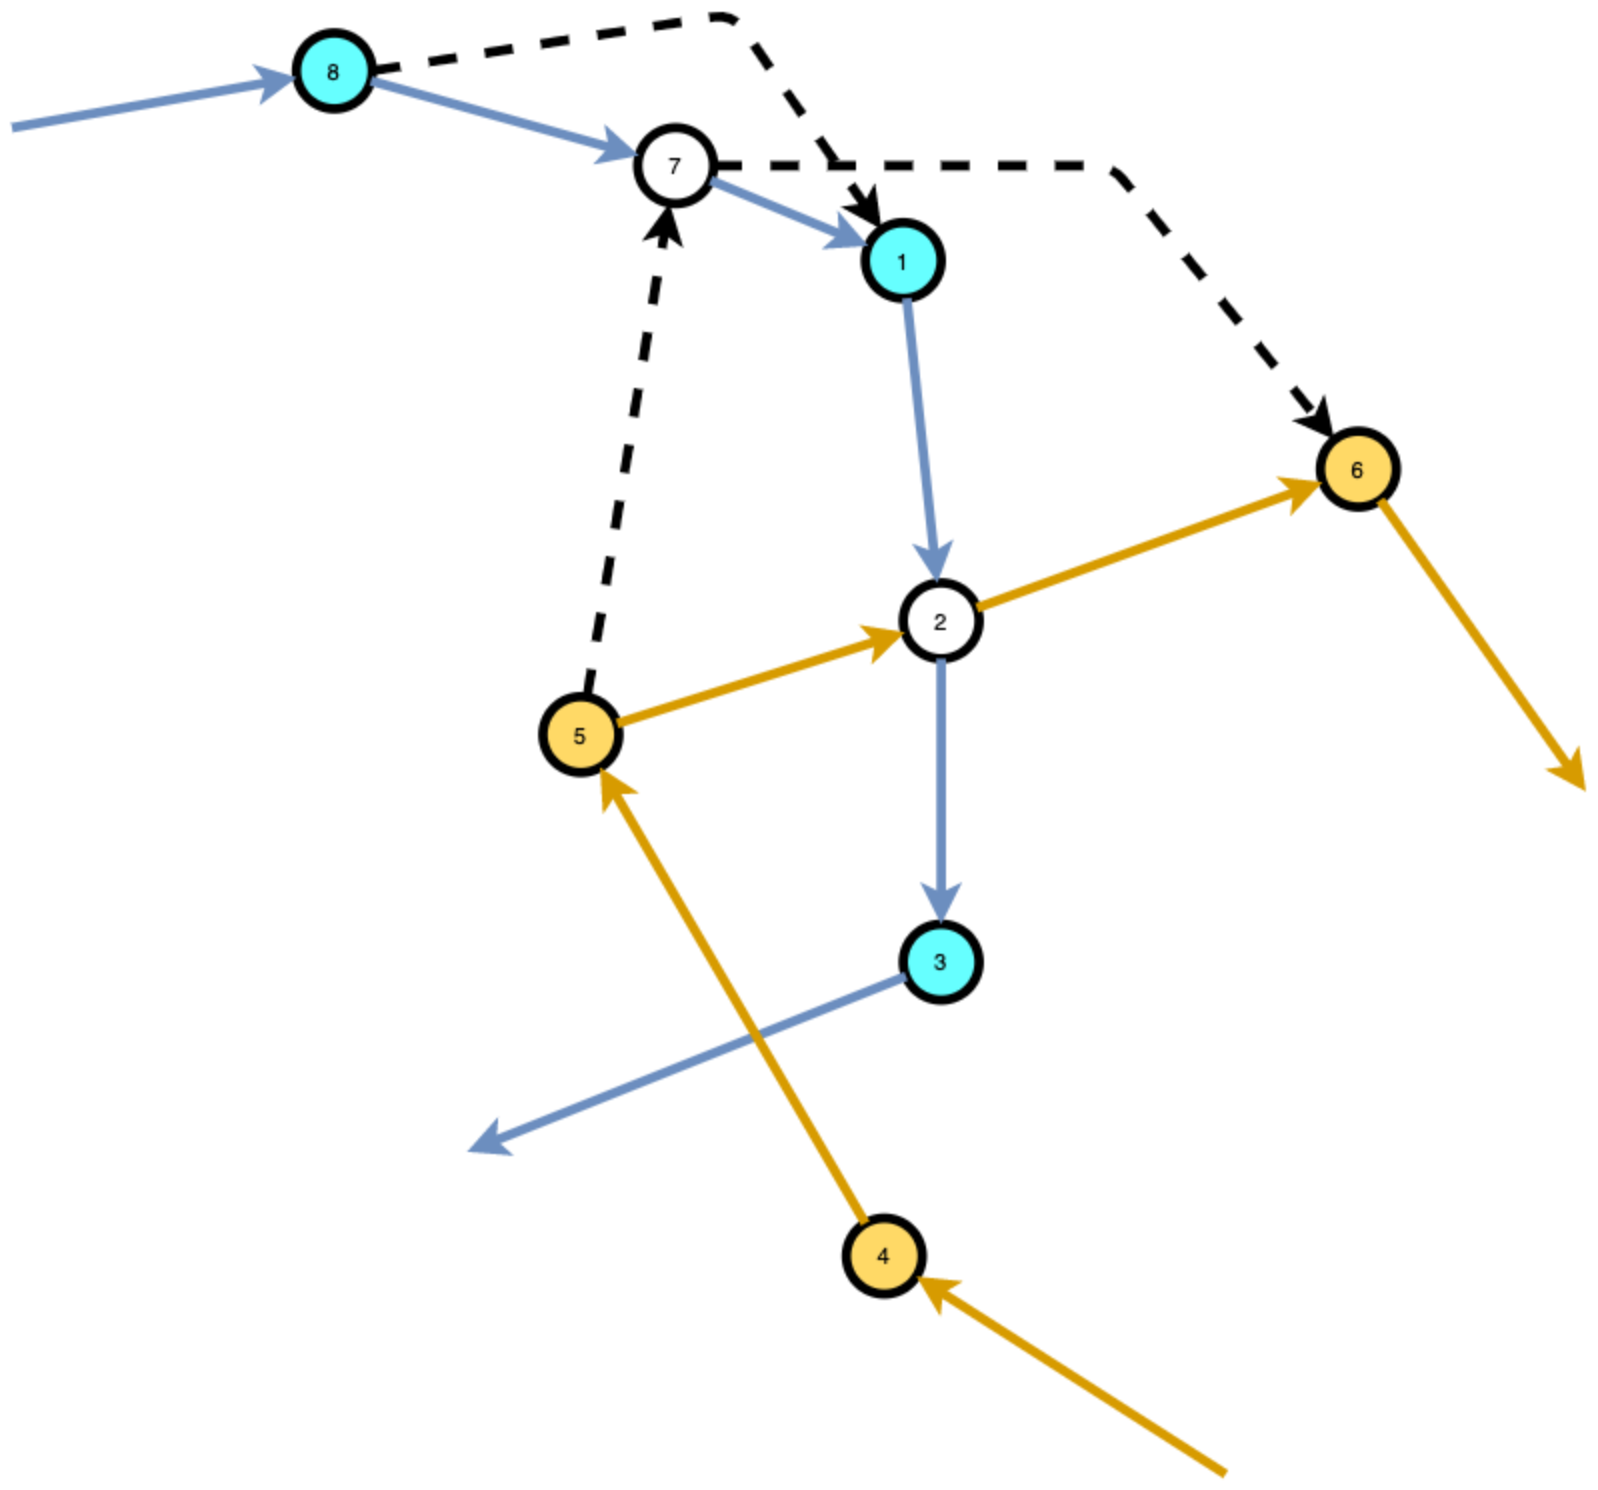
\includegraphics[width=0.8\textwidth]{assets/harder_conflict.png}
\caption{Harder Conflict}
\label{fig:harder_conflict}
\end{figure}

However, there is a long range effect that makes the problem harder. Consider the hard case in figure \ref{fig:harder_conflict}, we fix the path from $1 \to 3$ and again find the shortest path from $5 \to 6$ without inducing any conflict. But this time, the only path causes the path $8 \to 1$ to be rescheduled.

\begin{figure}[h!]
\centering
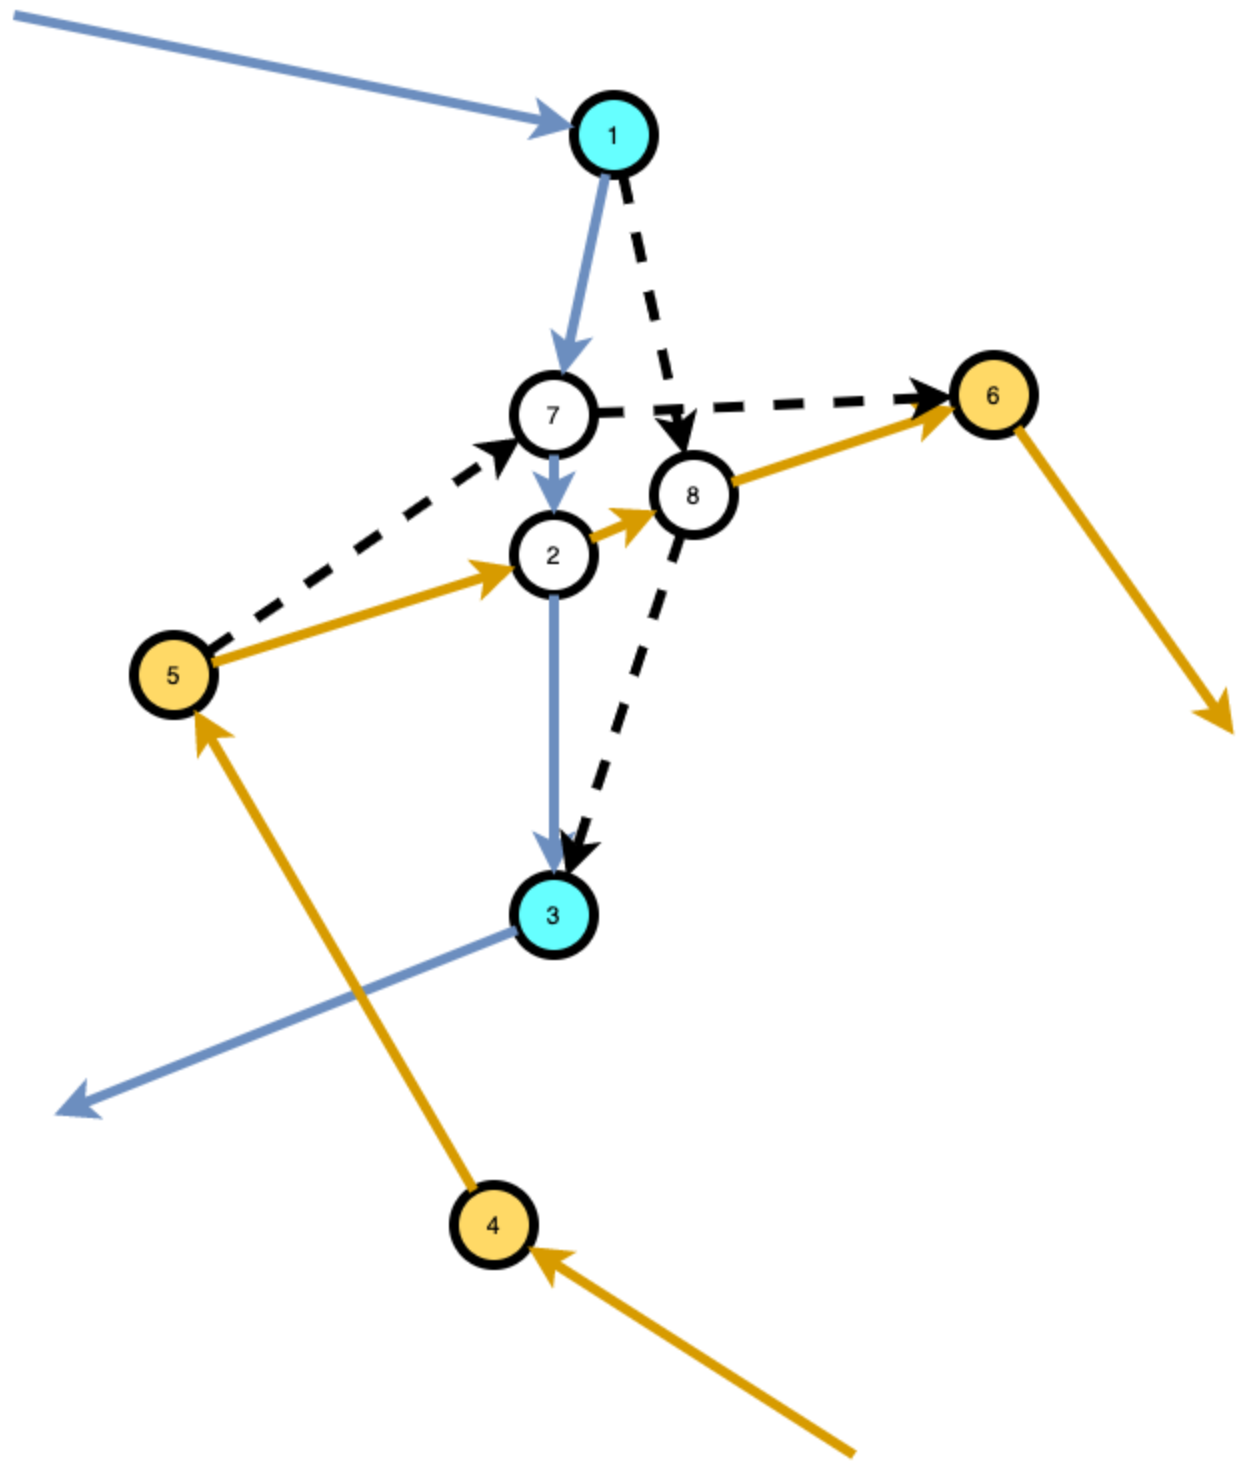
\includegraphics[width=0.8\textwidth]{assets/hardest_conflict.png}
\caption{Hardest Conflict}
\label{fig:hardest_conflict}
\end{figure}

In another case in figure \ref{fig:hardest_conflict}, we cannot pick any of the path from $1 \to 3$ or from $5 \to 6$ to be fixed while the solution still exists.

\subsection{Conflict Based Search}

Given a set of resources $R$ and a set of  $k$ agents $A$. Each agent associates with a subset of resources by the cost function $c: A \times P(R) \to \mathbb{R}$. Our goal is to find such $k$ disjoint subsets of $R$ associate with $k$ agents that minimize the total cost. 

In conflict-based search, we define a conflict tree with each node has 3 properties: \textbf{constraint}, \textbf{assignment} and \textbf{cost}. \textbf{constraint} is a set of constraints, \textbf{assignment} is the least cost function $a: A \to P(R)$ that uniquely assigns each agent to a subset of resources that satisfies the \textbf{constraint} and \textbf{cost} is the cost of \textbf{assignment}.
    
The branching rules is defined as follow:
    
(1) if there is no conflict (all subsets are disjoint), the node is a terminal node.
    
(2) Choose a conflict (a resource in common of more than one agent), branch-out to $m+1$ child nodes where $m$ is the number of agent taking that resource. In each of the first $m$ child nodes, add a constraint assigning the respective agent to take the resource. In last child node, add a constraint preventing all agents to take the resource.
    
To elaborate more on the branching rule (2), consider a node with properties as follow:
    
\fbox{\begin{minipage}{30em}
    
\textbf{constraint}: \{ $c_1$ \}
    
\textbf{assignment}: $a_1 \to \{r_1, r_2\},  a_2 \to \{r_2, r_3\}, a_3 \to \{r_2, r_4\}$
    
\textbf{cost}: some real number.
    
\end{minipage}}
    
    
Suppose we choose $r_2$ to branch-out, the first child node is:
    
\fbox{\begin{minipage}{30em}
    
\textbf{constraint}: \{ $c_1$, (assign $r_2$ to $a_1$) \}
    
\textbf{assignment}: least cost assignment satisfies the \textbf{constraint}
    
\textbf{cost}: some real number.

\end{minipage}}

The next two child node is constructed in the same manner by replacing the constraint on $a_1$ to $a_2$ and $a_3$ respectively.
    
The last child node is:
    
\fbox{\begin{minipage}{30em}
    
\textbf{constraint}: \{ $c_1$, (do not assign $r_2$ to any of \{$a_1$, $a_2$, $a_3$\}) \}
    
\textbf{assignment}: least cost assignment satisfies the \textbf{constraint}
    
\textbf{cost}: some real number.

\end{minipage}}
    
By splitting the conflict tree node in this way, there is no duplicate node since $m+1$ child nodes split from a parent node are mutually exclusive. In the case of $m=2$, the branching rules reduced to the method described in \cite{sharon2015conflict}.
    
Using best first search on the conflict tree guarantees to find the optimal assignment by the following two arguments:
    
\begin{lemma}[Complete]
Root node (empty \textbf{constraint}) permits the least cost terminal node if one exists.
\label{lemma:complete}
\end{lemma}
    
\begin{lemma}[Lower bound]
The cost of a conflict tree node is the lower bound of all terminal nodes it permits.
\label{lemma:lowerbound}
\end{lemma}
    
Lemma \ref{lemma:complete} can be proved by verifying the conflict tree is limited depth and for every branch-out, the least cost terminal node belongs to either one of the branches.
    
Lemma \ref{lemma:lowerbound} can be proved by contradiction since adding more constraints, the cost of a node cannot decrease.

\begin{theorem}[Completeness of CBS]
Conflict Based Search with best first search strategy guarantees to find the optimal assignment if one exists.
\end{theorem}

In conflict avoidance, we consider each tour as an agent, a subset of resources corresponding to a possible plan for that tour. Conflict can be modelled as a resource shared by more than one agent (same node, same edge). We further impose two additional branch-out rules that makes the algorithm capable to  explore its possible local advancement.

(1) \textbf{Transfer3}: the operation of transferring a node from a tour to another tour or itself.

(2) \textbf{Reverse}: reverse the direction of a tour.

Consider a series of POIs: $A \to B \to C \to D$. Let another tour occupied the path $C \to B$ (opposite direction). One possible strategy to is \textbf{reverse} the whole first tour, it becomes $D \to C \to B \to A$. Another strategy is the reschedule the first path to be $A \to C \to B \to D$, this rescheduled path can be obtained by \textbf{transfer3} of POI $C$ to edge $A \to B$